\documentclass{article}
\usepackage[utf8]{inputenc}
\usepackage{multicol}
\usepackage{geometry}
\usepackage{bm}
\usepackage{hyperref}
\usepackage{graphicx} % Required for including images
\usepackage[font=small,labelfont=bf]{caption} % Required for specifying captions to tables
%\usepackage{showframe} %This line can be used to clearly show the new margins

\newgeometry{vmargin={19mm}, hmargin={19mm,19mm}}   % set the margins
\graphicspath{ {./images/} }
\title{%
\vspace*{-2em}
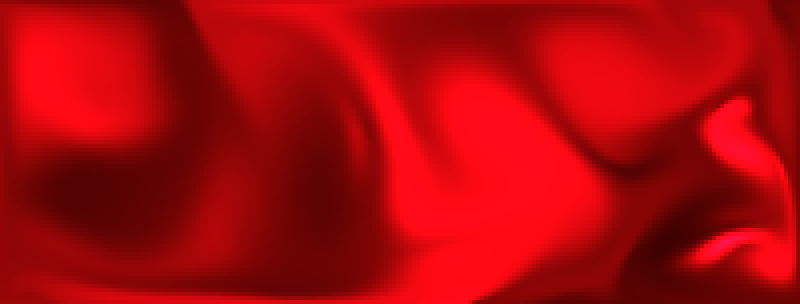
\includegraphics[width=\linewidth]{top}\\%
\textbf{Fluid Simulation Project Report}\\%
\large DH2323 Computer Graphics and Interaction}
\author{Pontus Asp}
\date{%
KTH Royal Institute of Technology\\%
2021-05-19}

\begin{document}
\maketitle
\begin{multicols}{2}

\section*{Abstract}
In this paper I present a simple fluid dynamics simulator based on the Navier-Stokes Equations and a paper by Jos Stam, but extended to include static objects the fluid can interact with in the simulation. This program can give a realistic looking simulation of fluids in real-time that could be used to demonstrate fluid movement where precise accuracy is not the main point, but where instead the visual quality is of higher importance.

\section{Introduction}
In the field of Computational Fluid Dynamics (CFD), incompressible fluids are simulated by a computer that will solve approximations to a set of differential equations which are called the Navier-Stokes Equations. In this project I simulated fluids in 2D with the technique of finite elements. But there are also other types of techniques, e.g. finite difference, finite volume and spectral methods. Some use cases for the Navier-Stokes equations could be to, for instance; Model weather, water flow, or air flow around objects etc. In computer simulated models, iterative solvers for approximating the differential equations are often used. In this project the Gauss-Seidel method will be used to iteratively approximate the systems of equations. The Navier-Stokes Equations:
\[
    \nabla \cdot \bm{u}=0,~~~~~~
    \rho\frac{d\bm{u}}{dt}=-\nabla p+\mu\nabla^2\bm{u}+\rho \bm{F}
\]
Where $u$ is the velocity vector field, $\rho$ is the density, $-\nabla p$ is the pressure, $\mu \nabla^2u$ is the viscosity and $F$ is external forces, e.g. gravity. The first equation $\nabla \cdot u=0$ is essentially describing that the mass is conserved within the fluid by making sure that the divergence of the velocity vector field is $0$. If we somewhere would have positive divergence then that would mean that the mass would be increasing at that point, and a negative divergence would mean that mass would disappear at that point. Since mass can't simply disappear or appear out of nothing the divergence has to be equal to $0$. The second equation corresponds closely with Newton's Second Law of Motion and describes the rules of movement of Newtonian fluids, like water. \cite{vcubingx}

\section{Related Work and Research}
When working on this project there are two main papers that I have used as inspiration when coding the simulation, one which talked about the material on an easier to understand, but less deep level, and one which went more into details but not far enough so that it was very hard to follow.\\
The first source is Jos Stam's paper Real-Time Fluid Dynamics for Games \cite{stam}. In this paper Stam both talks about some of the math behind implementing a real-time simulation of fluids and also goes through code for an actual implementation of a fluid simulation. The second source is Mike Ash's paper Fluid Simulation for Dummies \cite{ash}. This paper is similar to Stam's paper in some ways, and that is because the code here is based on Stam's code. The biggest difference in this paper compared to Stam's paper is that it is easier to read, as that was actually a primary goal for Ash when writing it. Using the combination of these two papers I planned out how I would want to write my implementation of the code and how I would be able to use the data from the simulation to create a viewer that could visualize it on the screen.

The after reading these papers I realized that the simulation uses two kinds of data when simulating the fluid, density and velocity. The density can be thought of as dye in the fluid, since the velocity is independent of the density values in the simulation. A real life example could be to put some food coloring in water, the water will still carry velocity through the fluid but we can not see how the fluid is moving in a closed space until we put some dye in it, and this is essentially what the density is representing. Something to keep in mind is that adding density to the simulation will not increase the mass or actual density of the fluid, it is simply for the purpose of keeping track of how things move around. The velocity is simply what describes the velocity in the water and how it will move around with time. So with this in mind I now know that I have two kinds of data that I can work with to visualize the simulation, the density (dye) and the velocity. Both of these papers also used the technique of finite elements by splitting the simulation up in a grid with discrete elements, which seemed like an easy way to work with the data so that is also what I decided to work with.

\section{Implementation and Results}
In this section I will present the implementation, thought process and results throughout the development of the project. I will also bring up some of the technologies that I used in this process. I also wrote a blog during development that is available online at: \url{https://github.com/pontusasp/fluid-simulation/blob/course/blog.md}

\subsection{Implementation of Viewer}
When implementing the viewer the first thing I had to decide was how I would like to present the graphics, and since I wanted to make a real-time simulation I wanted to have a window where the image would be updated in real-time. After researching different libraries and APIs I decided to use the SFML library since it had a small built in math library and was easy to use but still relatively low level.
I decided that I wanted to display the density values of the simulation and since the simulation is divided into a grid it would seem reasonable to display each cell as one pixel on the screen. But I wanted to be able to view the simulation in a larger scale so I started implementing a class that had a grid of squares which could be set to different colors. I called this class MeshImage. Each square in the grid consists of a quad defined by 4 vertices which we set the color of the square to. Each quad have their own set of vertices and we can therefore have sharp color changes between each cell, since they do not share any of the color data with their neighbours.
Later on in the development I also implemented another class that I would display on top of the MeshImage that visualized the velocity vectors as well. I did this by creating a field of arrows, where each arrow varies in size and color depending on the magnitude and also in direction depending on the velocity vector it was visualizing. I called this class VectorField.
Towards the very end of the project I also implemented static objects that could be added to the scene that was simply visualized in the MeshImage as a solid color different from the fluid, and also some buttons which could control and reset some parameters of the simulation.

\subsection{Simulation of Fluids}
The Navier-Stokes Equations are a good way to describe the rules of how motion can be applied to fluids, but does not give much information about how to simulate these motions \cite{inspecto}. Instead we have to make an algorithm that satisfies the rules of the Navier-Stokes Equations for our simulation.
\begin{itemize}
    \item Diffusion
    \item Advection
    \item Projection
    \item Setting bounds
\end{itemize}
These are the core steps of algorithm I have implemented, which will be explained in more detail in the following sections. Each of these steps will be used in conjunction to simulate discrete steps in time through the simulation. These steps are dependent on the previous time step, so we need to have a copy of the last time step at all times, so what we will do is have two sets of values for all data, one set that will store the current data and one set that stores the data from the last step.

\subsubsection{Diffusion}
The diffusion step is responsible for calculating how much data will spread out to neighbouring cells, the diffusion is used for both the velocity vectors and the density values. The diffusion works by solving a system of equations to make each cell converge towards the average value of its neighbours. This is the step in where we use the Gauss-Seidel method to iteratively approximate the system of equations to find the change in the cell during the current time step. Here, the precision of the outcome depends on the number of iterations we use for the Gauss-Seidel approximation and can therefore change the quality of our final simulation, so having a higher value of iterations here can be important if a more accurate simulation is desired. This project is more aimed towards the visual aspect of the simulation rather than accuracy, so the number of iterations is initially set to a pretty low value of 5 for the%
%
\end{multicols}%
\begin{center}
    \begin{minipage}{0.5\linewidth}
        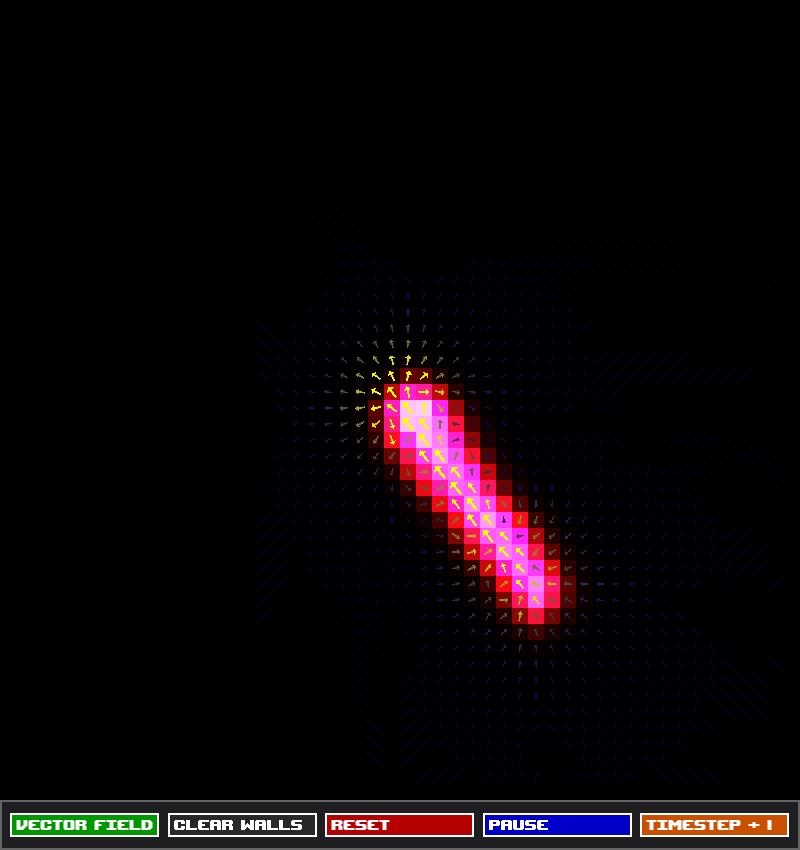
\includegraphics[width=4.1cm]{0_001f_diff_ts_1}
        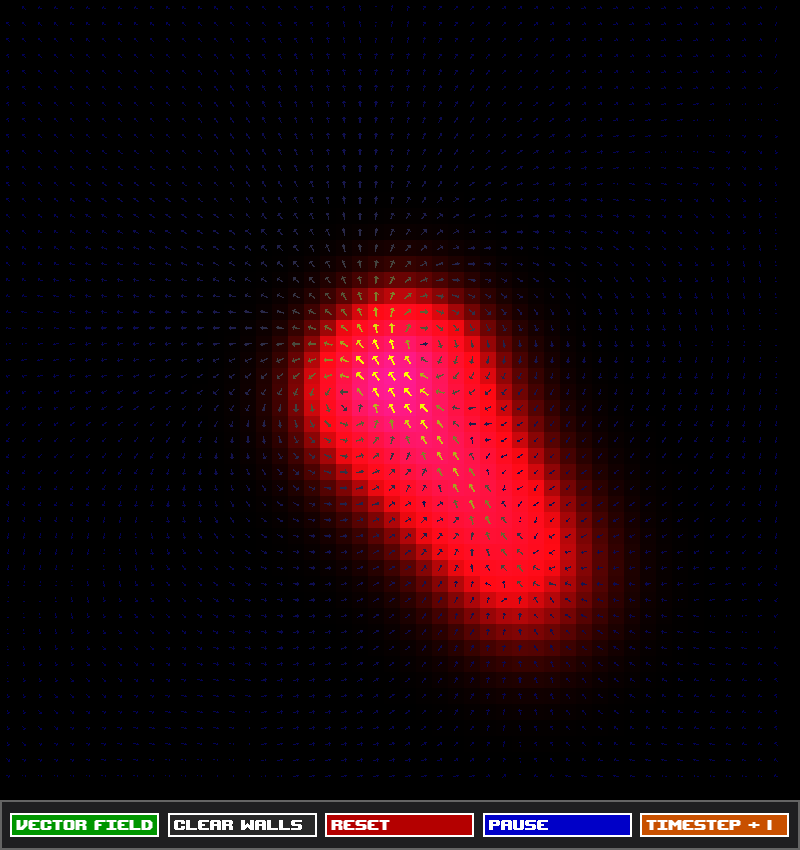
\includegraphics[width=4.1cm]{0_001f_diff_ts_20}
        \captionof{figure}{Diffusion $:= 10^{-3}$, Timestep 1 \& 20}
    \end{minipage}%
    \begin{minipage}{0.5\linewidth}
        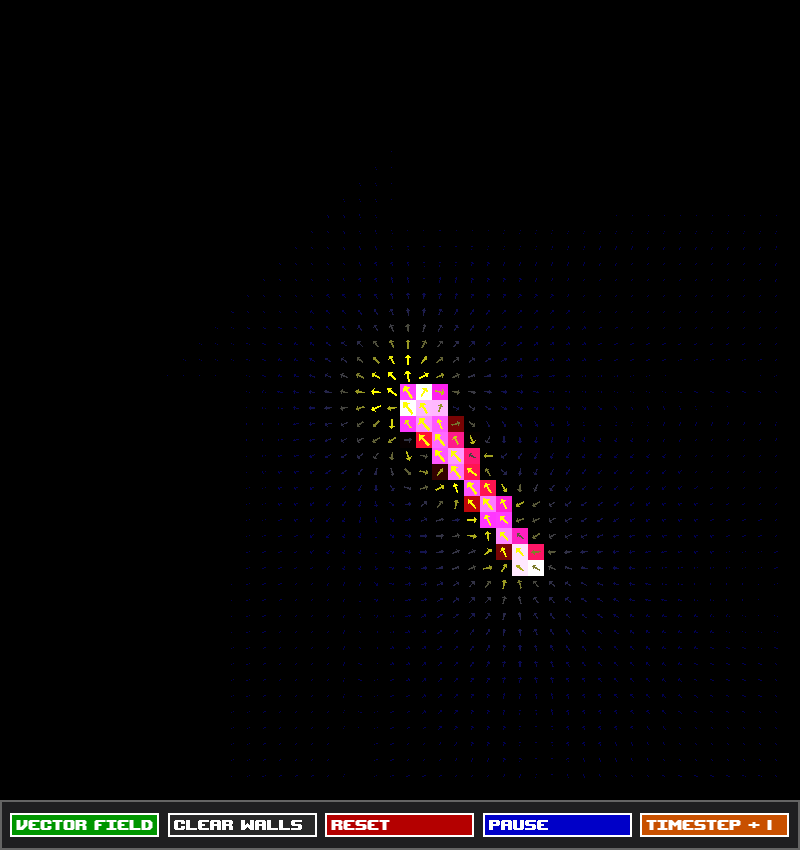
\includegraphics[width=4.1cm]{0_00000001f_diff_ts_1}
        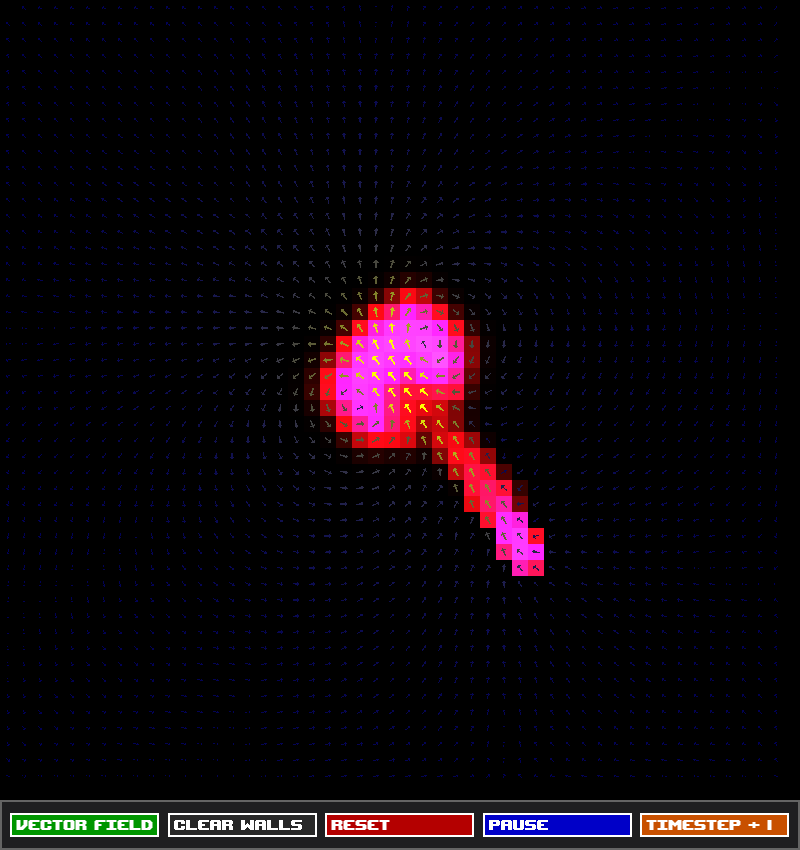
\includegraphics[width=4.1cm]{0_00000001f_diff_ts_20}
        \captionof{figure}{Diffusion $:= 10^{-8}$, Timestep 1 \& 20}
    \end{minipage}%
    \captionof*{figure}{Velocity is set with similar values in the direction left/up in both figures.}
\end{center}%
\begin{multicols}{2}%
\noindent%
simulation to have an acceptable frame rate. The diffusion step is done three (3) times per time step, one time per axis for the velocity values (velocities for the x and y axis since we are simulating in 2D), and one time for the density values.

When diffusing the velocity values the rate of convergence between the cells is dependent on the viscosity of the fluid, think of it as friction between the fluid particles. For instance, honey has a higher viscosity than water and will therefore not carry around the movement in the fluid as long as water would. When diffusing the density values in the simulation we are instead dependent on the given diffusion value of the density, i.e. a higher diffusion level makes the density spread out faster than a low diffusion level. For example, if we have a very high diffusion value the density would almost instantly spread out in the fluid to an even level, while a very low diffusion level would make the density almost not spread at all.

\subsubsection{Advection}
The advection step is responsible for calculating the movement of the data in the simulation, this step is dependent on the velocities in the simulation. A naive approach to this would probably be to trace where each cell we are currently calculating for end up and try to simply move our density there, but this poses two other problems. The first problem is that the velocity vectors are most likely not going to want to move the data to the exact center of the new cell, but closer to one side than the other, therefore we would have to spread out the data in a nice way between them. Then there is the other problem of that there might be more than one velocity vector that points to the same cell, and this adds even more complexity to the problem. What we do instead is find what data would move to our current cell if we go back in time and take the linearly interpolated value from the 4 cells surrounding the point we get. This way, we will always only have one point which will affect our current cell. This in turn also makes our simulation more stable.

Like with the diffusion step, we use the advection step for both of the velocity axes and also for the density values. At first it might seem weird that we move the velocity data as well, but think of it as the fluid particles with this velocity will actually move forwards and carry this velocity with them. A real life example would be that if you blow out a candle, the velocity of the air moves as it exits your mouth so that it can keep travelling forwards to the flame.

\subsubsection{Projection}
The projection step is important as it enforces the first equation of the Navier-Stokes Equation, $\nabla \cdot \bm{u}=0$. What the projection step does is to make sure that no part of the field has a divergence value of anything else than $0$, i.e. it takes care of conservation of mass. We can do this by finding the gradients at every point in our field and subtracting this from our current velocities, as this gives us a divergence free field according to the fundamental theorem of vector calculus. We can use a solution of a Poisson equation as we can use the Gauss-Seidel method again to approximate the solution to this system.

\subsubsection{Setting Bounds}
Something not mentioned in the previous steps, is that all other steps also utilizes this step, setting bounds. The bounds, which you might understand from the name, is the bounds of the simulation. In our case, the edges of the screen. This step makes sure that the borders of the simulation will counteract all forces applied to it, to make the simulation more physically accurate, as if it was contained in a box. The bounds will be set separately for each axis for the velocity and for the density values. The bounds work by flipping the sign of the incoming velocities in the same axis as it is currently bounding, and simply by copying the neighbouring values for the density bounding.

\subsubsection{Static objects}
I later also added static objects to the simulation. They worked similarly to the bounds and are set in the same function. The static objects relies on being at least 2x2 in size, so that they can act like the boundaries of the%
\end{multicols}%
\begin{center}
    \begin{minipage}{0.5\linewidth}
        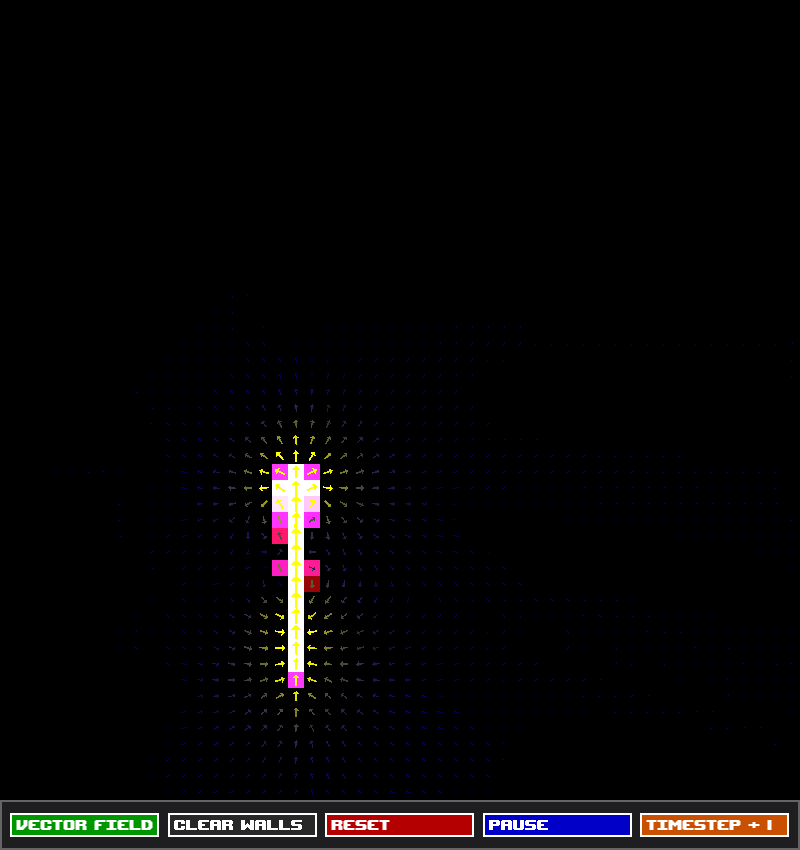
\includegraphics[width=4.1cm]{no_wall_ts_1}
        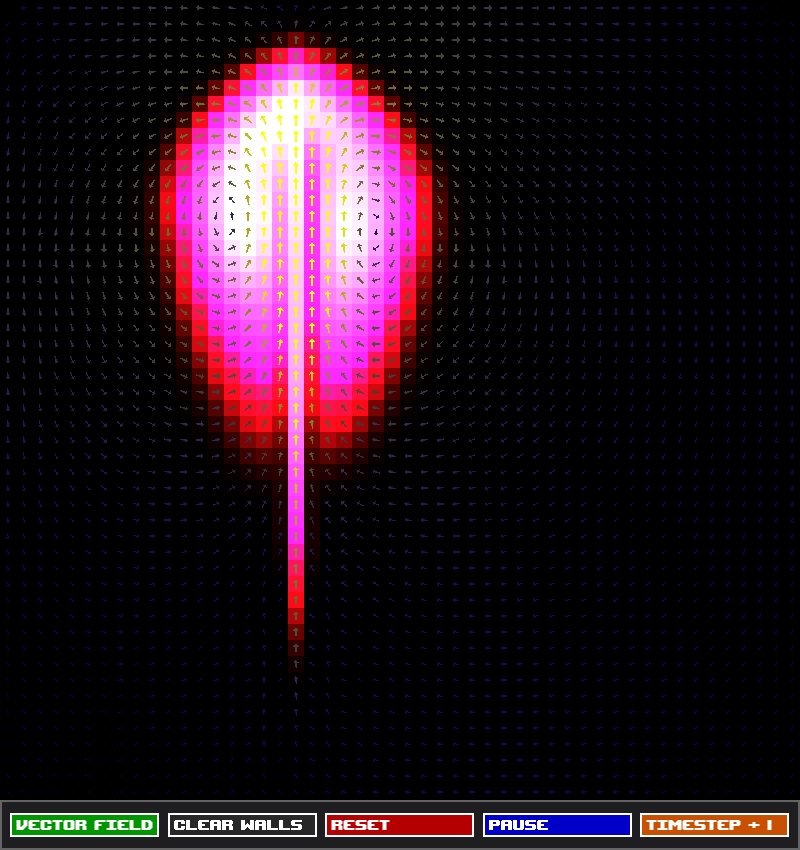
\includegraphics[width=4.1cm]{no_wall_ts_70}
        \captionof{figure}{Without static object, Timestep 1 \& 70}
    \end{minipage}%
    \begin{minipage}{0.5\linewidth}
        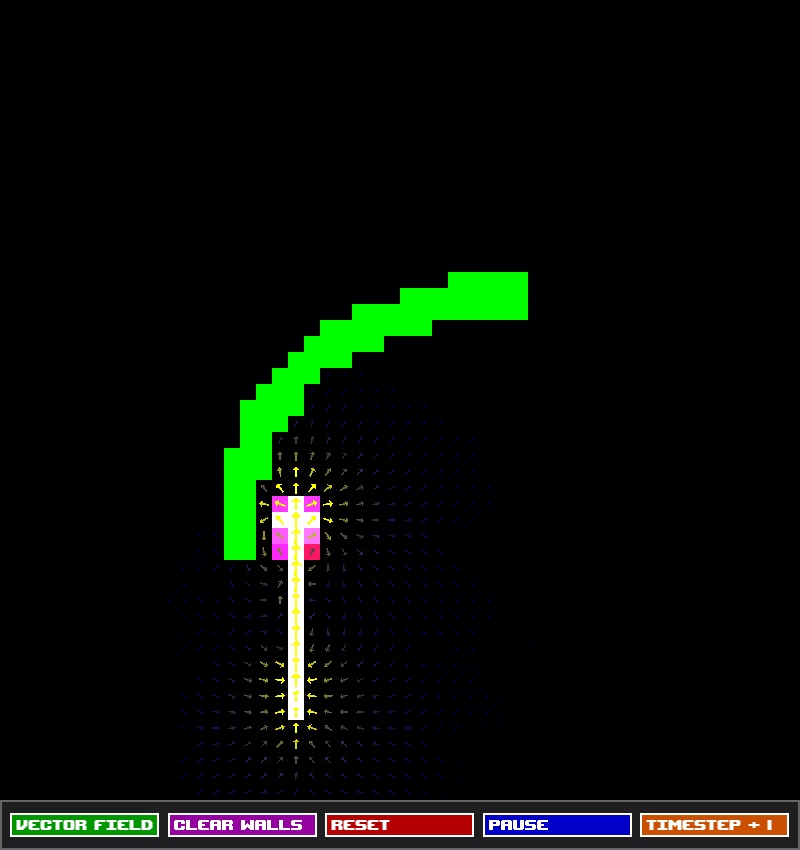
\includegraphics[width=4.1cm]{wall_ts_1}
        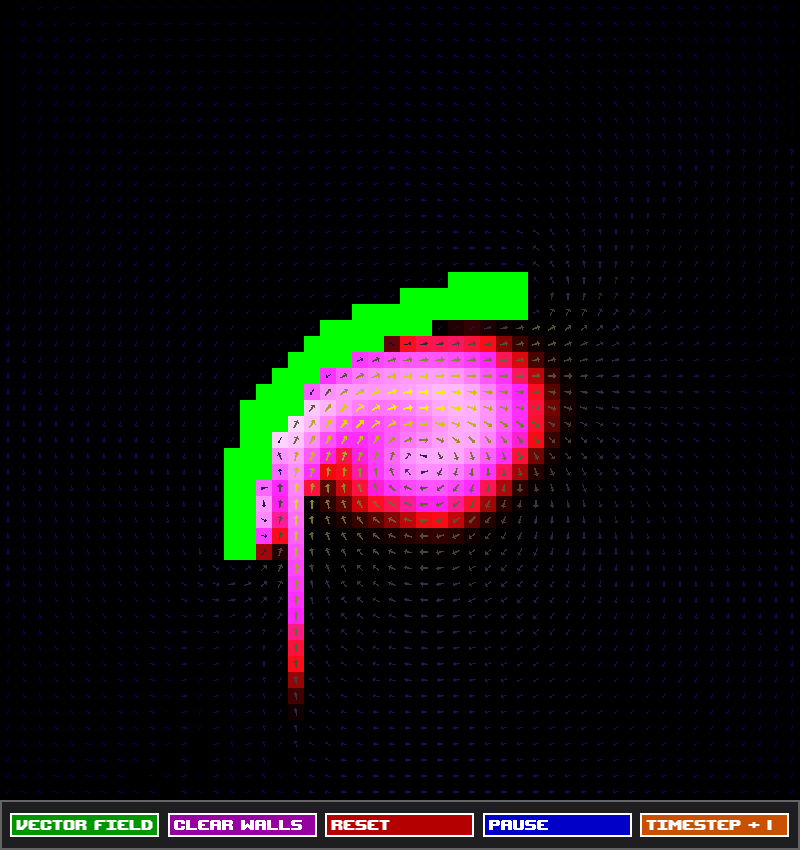
\includegraphics[width=4.1cm]{wall_ts_70}
        \captionof{figure}{With static object, Timestep 1 \& 70}
    \end{minipage}%
    \captionof*{figure}{Velocity is set with similar values upwards in both figures.}
\end{center}%
\begin{multicols}{2}%
\noindent%
screen by always making sure they can only have at least one side of each axis touch the fluids. By working like this all they have to do is check which side, if any, is a fluid cell. If has a fluid cell as a neighbour it will apply the same methods as we did for the boundaries at the edges of the screen. This implementation has a flaw though, and it is that these static objects do leak very slightly if the static objects are drawn in a diagonal line, but it is barely noticeable and with thicker static objects (like 3x3) it is even less prevalent, so much so that the densities does not look to be leaking at all. However when having a new simulation with no velocities at all, you can still see that with an enclosed space using these static objects, the velocities outside of them still change with a very small magnitude when new velocity is externally introduced inside the static objects borders. But considering how small the leaks are I felt like this can be considered like a working solution, since the entire simulation is approximated after all.
%
\subsection{From Data to Graphics}%
%
\begin{center}
    \begin{minipage}{\linewidth}
        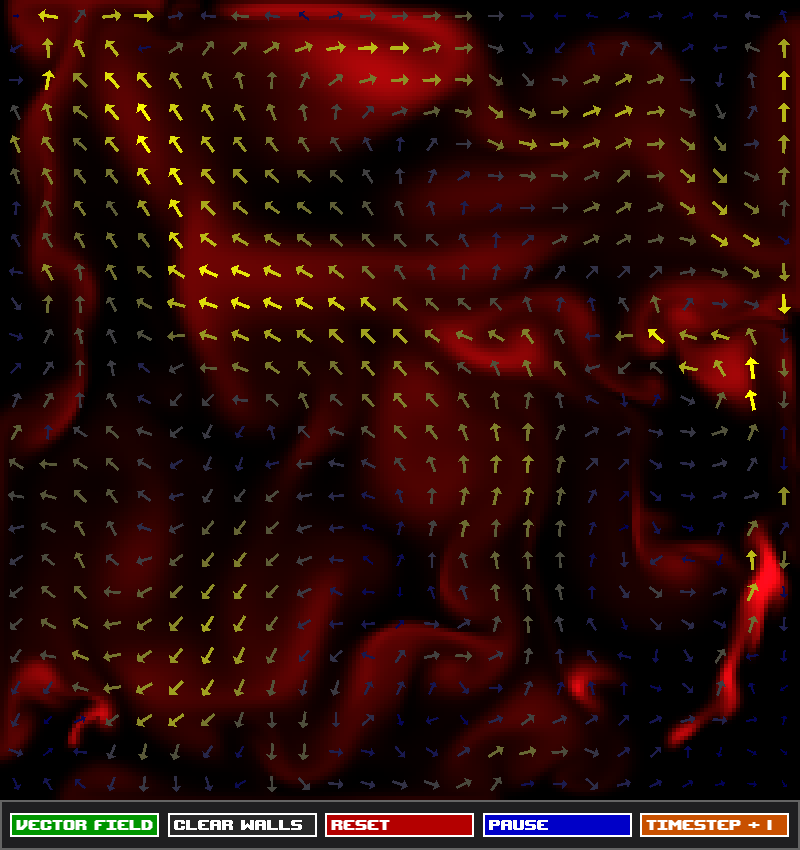
\includegraphics[width=4.15cm]{every_8th_field}
        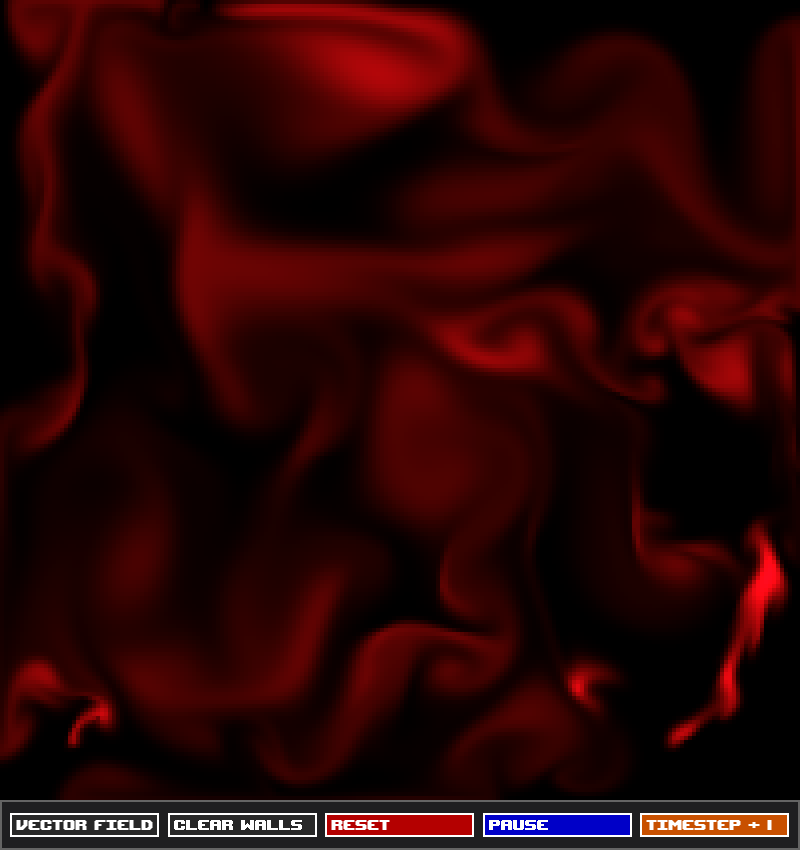
\includegraphics[width=4.15cm]{no_field}
        \captionof{figure}{Simulation with 200x200 grid with and without 25x25 VectorField.}
    \end{minipage}%
\end{center}%
\noindent
After simulating the fluid movement you also need a way to get that simulation to the screen. Earlier in this paper I mentioned that I programmed two classes, MeshImage and VectorField. What I did not mention is that the simulation itself is in a class called FluidSimulation. So for drawing the simulation to the screen there is a function in the FluidSimulation class that has a reference to a MeshImage object and a VectorField object. This function will then upon being called update both of these objects. Updating the MeshImage is done by iterating over every cell in the simulation and taking the value of the density and using this, simply linearly map it to a color from black, to red, to purple, to white. This is done very simply by multiplying the density value to each color channel and having the red channel statically set to 255 (before multiplication), the green channel to 10, and the blue channel to 20. After then multiplying these values they are capped at a max value of 255. Therefore we will get the fading between the different colors until we end up at white. Updating the VectorField is similar, but even more simple. The VectorField is designed to take two components which will add up to one final vector, this is where we iterate through all our velocity values and send them in pairs. The VectorField class then has enough information to know the magnitude and direction of the vectors and can then display them as arrows on the screen. The FluidSimulation class also has a paramenter which controls the scale of the VectorField class, i.e. if we have a scale of $1/4$ then the arrows will be distributed evenly over every fourth cell instead of every cell having their own vector arrow. The exact implementation of both of these classes are a bit out of scope for this paper, but both of them are pretty simple to implement as long as you have some basic knowledge about computer graphics.

\section{Future Work}
Things that would further improve this simulation would be to mainly optimize it, so that the gain in speed could be spent on making the simulation more accurate or have bigger scale than it currently does. In both of these cases, especially if bigger scale/higher resolution would be desired one viable option could be to offload a lot of the computation to the GPU since a lot of the computations has the potential to be heavily parallelized. I speculate that some parts of the code would have to be redesigned quite a lot though. Like the part of the code that is setting the bounds, since it is directly changing the data that it is computing with, and because it is accessing nearby cells. So there will be a dependency between the different kernels which would complicate things. Since the bounding function is called so often it would require the data to be transferred too often between the host and device to be effective if this function would not be rewritten to work on the device. Another option could be to change the grid to not have a static size, but have different level of detail depending on the amount of information (e.g. density) that exists in different parts of the simulation at different times and thereby save some computation power. Yet another option instead of GPU parallelization could be to simply make the code multi-threaded on the CPU, as it is right now only running on a single core.

Something that would be more easily implemented that would also improve the program would be to add more controls to the values of the simulation. As it is right now the values for diffusion and viscosity is hard-coded but could easily be implemented as sliders in the UI. Something slightly more challenging but very doable would be to also include an option to change the resolution (of the grid) of the simulation as that right now is also hard-coded.
%\columnbreak
%Column 2
\end{multicols}

\begin{thebibliography}{9}
\bibitem{stam}
J. Stam, “Real-Time Fluid Dynamics for Games”. Accessed: May 19, 2021. [Online]. Available: http://graphics.cs.cmu.edu/nsp/course/15-464/Spring11/papers/StamFluidforGames.pdf
\bibitem{ash}
M. Ash, “Fluid Simulation for Dummies”, (Mar. 13, 2006). https://www.mikeash.com/pyblog/fluid-simulation-for-dummies.html (accessed May 19, 2021).

\bibitem{vcubingx}
vcubingx, The million dollar equation (Navier-Stokes equations), (Jun. 06, 2020). Accessed: May 19, 2021. [Online Video]. Available: https://www.youtube.com/watch?v=Ra7aQlenTb8

\bibitem{inspecto}
Inspecto, But How DO Fluid Simulations Work?, (Dec. 16, 2020). Accessed: May 19, 2021. [Online Video]. Available: https://www.youtube.com/watch?v=qsYE1wMEMPA

\end{thebibliography}


\end{document}
